%%%%%%%%%%%%%%%%%%%%%%%%%%%%%%%%%%%%%%%%%
% Simple Sectioned Essay Template
% LaTeX Template
%
% This template has been downloaded from:
% http://www.latextemplates.com
%
% Note:
% The \lipsum[#] commands throughout this template generate dummy text
% to fill the template out. These commands should all be removed when 
% writing essay content.
%
%%%%%%%%%%%%%%%%%%%%%%%%%%%%%%%%%%%%%%%%%

%----------------------------------------------------------------------------------------
%	PACKAGES AND OTHER DOCUMENT CONFIGURATIONS
%----------------------------------------------------------------------------------------
\documentclass[12pt]{article} % Default font size is 12pt, it can be changed here

\usepackage{geometry} % Required to change the page size to A4
\geometry{a4paper} % Set the page size to be A4 as opposed to the default US Letter

\usepackage{graphicx} % Required for including pictures
\usepackage{subcaption}
\captionsetup{compatibility=false}
\usepackage{float} % Allows putting an [H] in \begin{figure} to specify the exact location of the figure
\usepackage{wrapfig} % Allows in-line images such as the example fish picture

\usepackage{mathtools}

\usepackage{hyperref}


\usepackage{fancyhdr}
\pagestyle{fancy}
\fancyhf{}
%\fancyhead[LE,RO]{Share\LaTeX}
\fancyhead[RE,LO]{Pixel-based Skin Color Detection Techniques}
\fancyfoot[CE,CO]{Master's in Computer Vision and Robotics, University of Burgundy}
\fancyfoot[LE,RO]{\thepage}
\renewcommand{\headrulewidth}{1.5pt}
\renewcommand{\footrulewidth}{1pt}
 

%\usepackage{lipsum} % Used for inserting dummy 'Lorem ipsum' text into the template

\linespread{1.1} % Line spacing

%\setlength\parindent{0pt} % Uncomment to remove all indentation from paragraphs

\graphicspath{{Pictures/}} % Specifies the directory where pictures are stored

% Defining tikz for flow chart
\usepackage{tikz}
\usetikzlibrary{shapes.geometric, arrows}

\tikzstyle{PointCloud} = [rectangle, rounded corners, minimum width=3cm, minimum height=1cm,text centered, text width=3cm, draw=black, fill=red!30]
\tikzstyle{Processes} = [rectangle, minimum width= 4.5cm, minimum height=1.1 cm,text centered, draw=black, fill=orange!30]
\tikzstyle{arrow} = [thick,->,>=stealth]


\usepackage{caption}
\usepackage{subcaption}
\usepackage{listings}
\usepackage{color} %red, green, blue, yellow, cyan, magenta, black, white
\definecolor{mygreen}{RGB}{28,172,0} % color values Red, Green, Blue
\definecolor{mylilas}{RGB}{170,55,241}

\lstset{language=Matlab,%
	basicstyle=\footnotesize\ttfamily,
	breaklines=true,%
	morekeywords={matlab2tikz},
	keywordstyle=\color{blue},%
	morekeywords=[2]{1}, keywordstyle=[2]{\color{black}},
	identifierstyle=\color{black},%
	stringstyle=\color{mylilas},
	commentstyle=\color{mygreen},%
	showstringspaces=false,%without this there will be a symbol in the places where there is a space
	numbers=left,%
	numberstyle={\tiny \color{black}},% size of the numbers
	numbersep=9pt, % this defines how far the numbers are from the text
	emph=[1]{for,end,break},emphstyle=[1]\color{red}, %some words to emphasise
	%emph=[2]{word1,word2}, emphstyle=[2]{style},    
}


\begin{document}

%----------------------------------------------------------------------------------------
%	TITLE PAGE
%----------------------------------------------------------------------------------------

\begin{titlepage}

\newcommand{\HRule}{\rule{\linewidth}{0.5mm}} % Defines a new command for the horizontal lines, change thickness here

\center % Center everything on the page

\textsc{\LARGE Image Processing Final Project}\\[1cm] % Name of your university/college
\textsc{\Large University of Burgundy}\\[0.8cm] % Major heading such as course name
\textsc{\large Master's in Computer Vision and Robotics}\\[0.5cm] % Minor heading such as course title
\textsc{\large (VIBOT \& MScV)}\\[0.8cm] % Minor heading such as course title

\HRule \\[0.8cm]
{ \huge \bfseries Pixel-based Skin Color Detection Techniques}\\[0.4cm] % Title of your document
\HRule \\[2cm]

\begin{minipage}{0.5\textwidth}
\begin{flushleft} \large
\emph{Group members:}\\
% Add names if you want
 %Yu \textsc{Liu}  \\ 
 Hassa ZAAL \\
 AbdelRahman ABUBAKR\\

\end{flushleft}
\end{minipage}
~
\begin{minipage}{0.4\textwidth}
\begin{flushright} \large
\emph{Supervisor:} \\
Prof. Desire Sedibe  % Supervisor's Name
\end{flushright}
\end{minipage}\\[3 cm]

%{\large \today}\\[1cm] % Date, change the \today to a set date if you want to be precise


\includegraphics{Logo}\\[0cm] % Include a department/university logo - this will require the graphicx package

% \vfill % Fill the rest of the page with whitespace

\end{titlepage}

%----------------------------------------------------------------------------------------
%	TABLE OF CONTENTS 
%----------------------------------------------------------------------------------------

 \tableofcontents % Include a table of contents

\newpage % Begins the essay on a new page instead of on the same page as the table of contents 

%----------------------------------------------------------------------------------------
%	INTRODUCTION
%----------------------------------------------------------------------------------------
\section{Introduction} % Major section

Human skin color has been used and proved to be an effective feature in many applications such as human face detection, hand tracking, image content filtering, content-aware video compression and many more. In this project we implemented the algorithms mentioned in the paper "A Survey on Pixel-Based Skin Color Detection Techniques" by Vladimir Vezhnevets, Vassili Sazonov, and Alla Andreeva.

\subsection{UCI skin segmentation data set}

The Authors of the paper mentioned using the Compaq skin database for comparing the results of all algorithms. However, we could not find any source for the Compaq database, therefore we decided to use the UCI skin segmentation dataset, provided by Center for Machine Learning and Intelligent Systems at University of California, Irvine. the dataset can be downloaded from here:
\href{https://archive.ics.uci.edu/ml/datasets/Skin+Segmentation}{https://archive.ics.uci.edu/ml/datasets/Skin+Segmentation} \\

According to the dataset website, the skin dataset is collected by randomly sampling B,G,R values from face images of various age groups (young, middle, and old), race groups (white, black, and asian), and genders obtained from FERET database and PAL database. Total learning sample size is 245057; out of which 50859 is the skin samples and 194198 is non-skin samples.\\

This dataset is of the dimension 245057 * 4 where first three columns are B,G,R values and fourth column is of the class labels (decision variable y), in the dataset file Skin colors are labeled as number 1 and Nonskin elements as 2.

\subsection{Dataset visualization}
First step to start any project with big amount of data, is to visualize this data to see its distribution and roughly expect the behavior of your algorithms. for our data set, we wrote a simple code Plot-Dataset.py that plots skin data in blue, and nonskin in red, the 2 axes are the Cb and Cr components of the colors. Figure shows the visualization of the dataset. 

\begin{figure}[H]
		\centering
		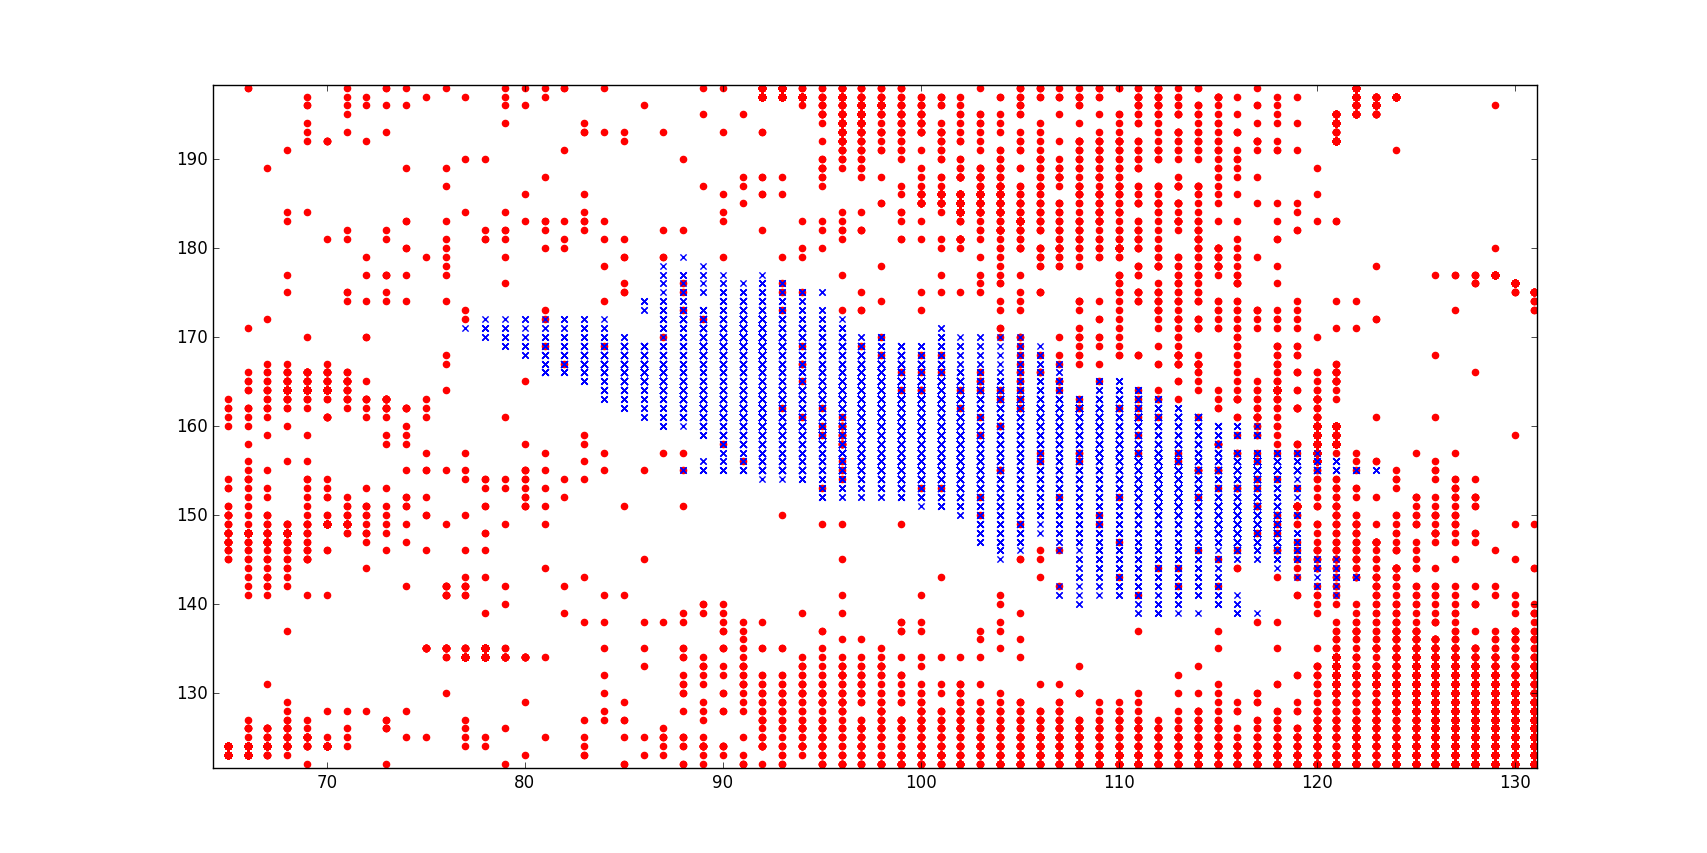
\includegraphics[width=\textwidth]{Skin-Nonskin-zoomed.png}
		\caption{UCI Data set visualization}	
\end{figure}

\subsection{How to run ?}
For the code implementation we used Python 3.5, with some help from Scikit-Learn 0.18.1 library when needed. We put all the algorithms in different files, and different directories, so for running any code, you can use any python IDE, or by Linux terminal change the directory for the code directory, then write:

\hspace*{\fill}
        Python  FileName.py
\hspace*{\fill} \\


%\\
All source code is available on Github Repository:
\href{https://github.com/abdelrahman-gaber/Pixel-based-Skin-Color-Detection}{https://github.com/abdelrahman-gaber/Pixel-based-Skin-Color-Detection } 


\subsection{Explicitly defined skin region} 


\section{Non-parametric skin distribution modeling} % Major section
The final goal of skin color detection is to build a decision rule, that will discriminate between skin and non-skin pixels. This is usually accomplished by introducing a metric, which measures distance (in general sense) of the pixel color to skin tone. The type of this metric is defined by the skin color modeling method. the paper differentiated between many types of modeling, the most important two of them are Non-parametric and parametric skin modeling techniques.\\

The key idea of the non-parametric skin modelling methods is to es-
timate skin color distribution from the training data without deriving an explicit model of the skin color. The result of these methods sometimes is referred to as construction of Skin Probability Map (SPM).





\subsection{Bayes Classifier} 



\section{Parametric skin distribution modeling} % Major section


\subsection{Single Gaussian model } 

\subsection{Gaussian Mixture Model (GMM)}

\subsection{Elliptic boundary model}







\appendix
\addcontentsline{toc}{section}{Appendices}
\section*{Appendices}
\section{Normalization code}

In this appendix, we show the code of the normalization step. this code is tested with all the face images, and the results are attached with the code. 

\begin{lstlisting}	

\end{lstlisting}

\section{PCA Code}


%----------------------------------------------------------------------------------------
%	BIBLIOGRAPHY >> If there are references
%----------------------------------------------------------------------------------------
%\begin{thebibliography}{99} % Bibliography - this is intentionally simple in this template

%\bibitem[Figueredo and Wolf, 2009]{Figueredo:2009dg} Figueredo, A.~J. and Wolf, P. S.~A. (2009).

%\newblock Assortative pairing and life history strategy - a cross-cultural  study.
%\newblock {\em Human Nature}, 20:317--330.
 
%\end{thebibliography}

%----------------------------------------------------------------------------------------

\end{document}